% Part: history
% Chapter: set-theory
% Section: limits

\documentclass[../../../include/open-logic-section]{subfiles}

\begin{document}

\olfileid[pt]{his}{set}{limits}	

\olsection{Definição Rigorosa de Limites}

Hoje em dia, a solução padrão ao problema anterior é livrar-se dos
infinitesimais. Eis como.

Já vimos que, à medida que $\beta$ fica menor, obtemos melhores aproximações do
gradiente. De fato, à medida que $\beta$ se aproxima arbitrariamente de $0$, o
valor de $f'(c)$ ``tende sem limite'' para o gradiente que queremos. Assim,
em vez de considerar o que acontece \emph{em} $\beta = 0$, precisamos
apenas considerar a \emph{tendência} de $f'(c)$ quando $\beta$ se aproxima de $0$. 

Posto deste modo, o desafio geral é dar sentido a afirmações desta forma:
\begin{center}
À medida que $x$ se aproxima de $c$, $g(x)$ tende sem limite para $\ell$. 
\end{center}
que podemos escrever de forma mais compacta assim:
\[
\lim_{x \rightarrow c}g(x) = \ell.
\]
No século XIX, sobre trabalho anterior de Cauchy, Weierstrass
deu uma definição perfeitamente rigorosa desta expressão. A ideia
é, de fato, que podemos tornar $g(x)$ tão próxima quanto queiramos de~$\ell$, 
tornando $x$ adequadamente próximo de~$c$. Mais precisamente, estipulamos que
$\lim_{x \rightarrow c} g(x) = \ell$ significará:
\[
(\forall\epsilon > 0)(\exists \delta > 0)\forall x \left(|x - c| < \delta \lif |g(x) - \ell| < \epsilon \right).
\]
As barras verticais indicam aqui valor absoluto. Isto é, $|x| = x$
quando $x \geq 0$, e $|x| =-x$ quando $x < 0$; pode representar-se
\emph{essa} função como se segue:
\begin{center}
	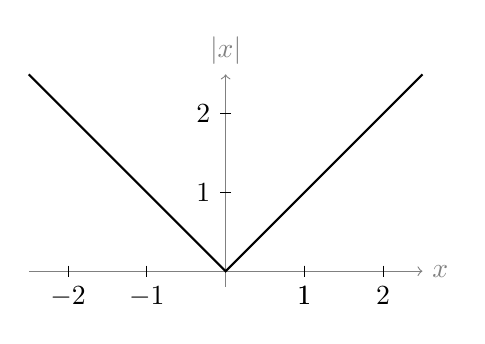
\begin{tikzpicture}[scale=1]
	\draw[->, gray] (-2.5,0) -- (2.5,0) node[right] {$x$};
	\draw[->, gray] (0,-.2) -- (0,2.5) node[above] {$|x|$};
	
	\foreach \x/\xtext in {-2/-2, -1,1, 1/1, 2/2}
	\draw[shift={(\x,0)}] (0pt,2pt) -- (0pt,-2pt) node[below] {{$\xtext$}};
	
	\foreach \y/\ytext in {1/1, 2/2}
	\draw[shift={(0,\y)}] (2pt,0pt) -- (-2pt,0pt) node[left] {{$\ytext$}};
	
	\draw[thick] (-2.5, 2.5)--(0,0)--(2.5, 2.5);
	\end{tikzpicture}
\end{center}
A definição diz portanto, grosso modo, o seguinte: pode tornar o seu ``erro'' inferior
a $\epsilon$ (isto é, $|g(x) - \ell| < \epsilon$) escolhendo
argumentos que distem no máximo $\delta$ de~$c$ (isto é, $|x -
c| < \delta$). 

Tendo definido a noção de limite, podemos usá-la para evitar por completo os
infinitesimais, estipulando que o gradiente de $f$ em $c$
é dado por:
\[
	{f}'(c) = \lim_{x \rightarrow 0}\left(\frac{f(c +x) - f(c)}{x}\right) \text{ quando um limite existe}.
\]
É importante, no entanto, compreender por que a nossa definição precisa da
ressalva ``quando um limite existe''. Para um exemplo simples, considere
$f(x) = |x|$, cujo gráfico acabamos de ver. Evidentemente, $f'(0)$ está
mal definida: se nos aproximamos de $0$ ``pela direita'', o gradiente é
sempre $1$; se nos aproximamos ``pela esquerda'', o gradiente é
sempre $-1$; logo o limite não está definido. Como tal, podemos acrescentar que uma
função~$f$ é \emph{diferenciável} em~$x$ se e só se tal limite existe.

Já vimos como tratar a diferenciação usando a noção de
\emph{limite}. Podemos usar a mesma noção para definir a ideia de função
\emph{contínua}. (Bolzano tinha, com efeito, percebido isto já por
1817.) O tratamento Cauchy--Weierstrass da continuidade é o seguinte.
Grosso modo: uma função~$f$ é contínua (num ponto) desde que, ao
exigir um certo grau de precisão relativamente à saída da
função, se possa garantir essa precisão insistindo num certo grau de
precisão relativamente à entrada da função. Mais precisamente: $f$ é
contínua em $c$ desde que, à medida que $x$ tende para zero, a diferença
entre $f(c + x)$ e $f(c)$ tenda para $0$. De outro modo: $f$
é \emph{contínua} em $c$ se e só se $f(c) = \lim_{x \rightarrow c} f(x)$. 

Ir mais longe levar-nos-ia apenas para a análise real, quando o nosso
tema é a teoria dos conjuntos. Por isso, agora devemos fazer uma pausa e enunciar a
moral. Durante o século XIX, os matemáticos aprenderam a passar
sem infinitesimais, invocando uma noção rigorosamente definida de
\emph{limite}.

\end{document}
